% =========================================================================
% Subsubsection: End-to-End Cross-Institution Access Latency Comparison
%
% Drop this file into your paper with % =========================================================================
% Subsubsection: End-to-End Cross-Institution Access Latency Comparison
%
% Drop this file into your paper with % =========================================================================
% Subsubsection: End-to-End Cross-Institution Access Latency Comparison
%
% Drop this file into your paper with % =========================================================================
% Subsubsection: End-to-End Cross-Institution Access Latency Comparison
%
% Drop this file into your paper with \input{cross-institution-latency-section}.
%
% Required preamble (add to your main .tex if not already present):
%   \usepackage{booktabs}
%   \usepackage{multirow}
%   \usepackage{graphicx}
%
% Figure dependency:
%   cross_institution_latency.pdf  (regenerate with: python3 plot_cross_institution_latency.py)
%   Place the .pdf alongside this .tex (or under your figs/ directory)
%   and update the \includegraphics path below if needed.
% =========================================================================

\subsubsection{End-to-End Cross-Institution Access Authorization and Verification Latency}
\label{sec:eval-e2e-cross-institution}

We evaluate the end-to-end latency of cross-institution Electronic
Health Record (EHR) access authorization and verification across five
architectural designs: a centralized OIDC consent registry
(\textit{OIDC-only}), a private-key DID/VC presentation model
(\textit{Private-key DID/VC}), an ACTION-EHR-inspired patient-centric
on-chain access-control baseline (\textit{ACTION-EHR-inspired}), a
zkLogin-driven on-chain access-grant baseline (\textit{zkLogin-only}),
and our proposed \textit{zkEHR} system, which combines DID-bound
on-chain AccessGrant objects, multi-authority salt derivation, and
zkLogin authentication. For the two zkLogin-based architectures we
report two operational modes: \textit{no-session} (the patient's
zkLogin credentials are derived from scratch on every access) and
\textit{session-reuse} (the patient establishes a zkLogin session once
and reuses the cached
$(\text{ephemeral key},\, \text{proof},\, \text{addressSeed},\,
\text{maxEpoch})$ tuple until the bound \texttt{maxEpoch} expires).

\paragraph{Experimental setup.}
All chain-touching baselines target Sui Devnet through the same Sui
Move \texttt{access\_grant} package, deployed once and shared across
baselines for fairness. The benchmarking host is a single Amazon EC2
instance in \texttt{us\nobreakdash-east\nobreakdash-1}, geographically
close to Sui's GCP-hosted devnet RPC endpoint
\texttt{fullnode.devnet.sui.io} ($\approx$1.5\,ms TCP RTT). For each
baseline we record 100 measured runs preceded by 10 warm-up runs that
are dropped from statistics. High-resolution timing uses
\texttt{process.hrtime.bigint()} (nanosecond resolution). Failed runs
are reported separately and excluded from latency percentiles. Sui
transactions use the \texttt{WaitForEffectsCert} submission semantics;
queries that target freshly-created objects use bounded retries to
absorb fullnode indexer lag (the wait is included in
\texttt{access\_grant\_query\_ms}, matching realistic e2e cost). For
zkEHR, multi-authority salt derivation uses $N{=}4$ co-located
authorities behind a parallel fan-out and a SHA-256 merge to a 128-bit
salt.

\paragraph{Results.}
Table~\ref{tab:e2e-cross-institution-latency} reports per-phase and
end-to-end latency for each baseline.
Figure~\ref{fig:e2e-cross-institution-latency} visualizes the
distribution on a logarithmic scale to span the four orders of
magnitude across baselines. We make five observations:

\begin{enumerate}
\item \textbf{Private-key DID/VC} achieves the lowest end-to-end
latency ($9.1$\,ms) because the patient signs the consent VC locally
and Hospital A issues a single chain query for DID resolution. However,
it provides no keyless recovery, no on-chain consent revocation
visibility, and no IdP-anchored identity binding.

\item \textbf{OIDC-only} attains the lowest \textit{access-side}
latency ($0.7$\,ms) since consent is centrally stored, but it incurs a
$255.6$\,ms federated-login cost on every grant operation because it
has no on-chain artifact and the consent registry is owned solely by
Hospital~A.

\item In \textbf{no-session mode}, both zkLogin-only ($3498.3$\,ms) and
zkEHR ($3553.3$\,ms) are dominated by the Mysten devnet prover request
that produces the Groth16 proof ($\approx$$2.8$\,s, $\approx$$80\%$ of
the end-to-end cost). Multi-authority salt with $N{=}4$ authorities
adds only $5.4$\,ms over single-authority salt, $0.15\%$ of the
no-session end-to-end cost.

\item In \textbf{session-reuse mode}, zkLogin-only ($466.9$\,ms),
zkEHR ($456.5$\,ms), and ACTION-EHR-inspired ($514.7$\,ms) converge
because they share the same dominant cost: a Sui transaction
submission ($\approx$$190$\,ms with \texttt{WaitForEffectsCert}) plus
one or two \texttt{getObject} round-trips ($\approx$$160$\,ms each,
including fullnode index lag for freshly-created objects).

\item \textbf{zkEHR adds only $5.7$\,ms} of B-DID resolution on top of
zkLogin-only-reuse---a $1.2\%$ access-time overhead---in exchange for
full DID-resolved authorization, portable consent semantics, and
keyless recovery support.
\end{enumerate}

% --------------------------- Table -----------------------------------------
\begin{table*}[!t]
\caption{End-to-end cross-institution access latency across five
architectures (mean$\,\pm\,$std., $n{=}100$ measured runs each, on Sui
Devnet via Amazon EC2 us-east-1). \textit{ns}=no-session;
\textit{r}=session-reuse.}
\label{tab:e2e-cross-institution-latency}
\centering
\renewcommand{\arraystretch}{1.25}
\begin{tabular}{l rrr l}
\toprule
\textbf{Baseline} & \textbf{Grant phase (ms)} & \textbf{Access phase (ms)} & \textbf{End-to-end (ms)} & \textbf{Notes} \\
\midrule
OIDC-only                       & $\phantom{0}255.6 \pm \phantom{00}27.4$ & $\phantom{000}0.7 \pm \phantom{0}0.1$  & $\phantom{0}256.3 \pm \phantom{00}27.5$ & Centralized consent DB \\
Private-key DID/VC              & $\phantom{0000}0.6 \pm \phantom{000}0.1$ & $\phantom{000}8.4 \pm \phantom{0}1.3$  & $\phantom{0000}9.1 \pm \phantom{000}1.3$  & Local VC sign; 1 DID-resolve RPC \\
ACTION-EHR-inspired             & $\phantom{0}340.8 \pm \phantom{00}80.3$ & $\phantom{0}171.1 \pm 78.4$ & $\phantom{0}514.7 \pm \phantom{0}117.9$ & On-chain grant + verify \\
zkLogin-only (\textit{ns})      & $3327.1 \pm 325.6$ & $\phantom{0}171.2 \pm 52.6$ & $3498.3 \pm \phantom{0}339.9$ & Fresh OIDC + prover per access \\
zkLogin-only (\textit{r})       & $\phantom{0}294.9 \pm \phantom{00}44.6$ & $\phantom{0}172.0 \pm 59.0$ & $\phantom{0}466.9 \pm \phantom{00}80.3$ & Cached zkLogin proof; 1 chain RPC \\
\textbf{zkEHR} (\textit{ns})    & $\mathbf{3364.6 \pm 350.0}$            & $\mathbf{188.6 \pm 61.3}$ & $\mathbf{3553.3 \pm 356.3}$ & Multi-auth salt + DID-bound \\
\textbf{zkEHR (ours,~\textit{r})} & $\mathbf{289.7 \pm \phantom{00}37.7}$ & $\mathbf{166.7 \pm 59.9}$ & $\mathbf{456.5 \pm \phantom{00}67.5}$ & Cached + DID-bound; 2 chain RPCs \\
\bottomrule
\end{tabular}
\end{table*}

% --------------------------- Figure ----------------------------------------
% Figure rendered by plot_cross_institution_latency.py (matplotlib);
% regenerate via: python3 plot_cross_institution_latency.py
\begin{figure*}[!t]
\centering
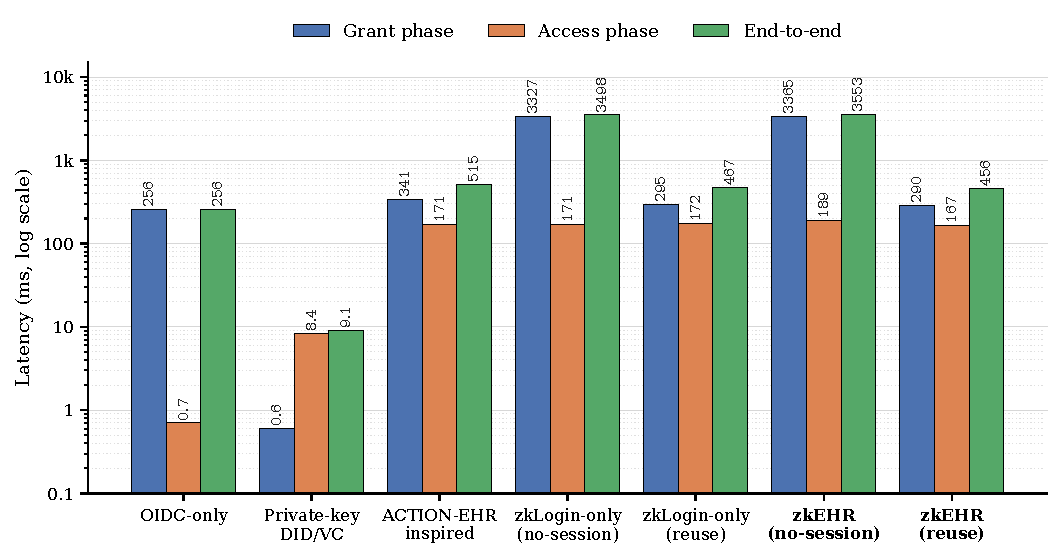
\includegraphics[width=0.95\textwidth]{cross_institution_latency.pdf}
\caption{End-to-end cross-institution access latency across five
architectures (mean of $n{=}100$ measured runs, log scale).
\textit{(no-session)} denotes that the patient performs the full
zkLogin authentication on every access; \textit{(reuse)} denotes that
the patient establishes a zkLogin session once and reuses the cached
proof for subsequent accesses within the bound \texttt{maxEpoch}
window. The proposed zkEHR variants are highlighted in bold on the
$x$-axis. zkEHR (reuse) matches the simpler on-chain access-control
baselines in per-access cost while delivering keyless recovery,
OIDC-anchored identity binding, and DID-portable consent.}
\label{fig:e2e-cross-institution-latency}
\end{figure*}

\paragraph{Cost of the zkEHR security guarantees.}
The defining features of zkEHR---multi-authority salt derivation for
keyless DID recovery and DID-bound AccessGrants for portable consent
authorization---are visible in two complementary regimes. In
no-session mode (every access pays a fresh zkLogin authentication),
multi-authority salt with $N{=}4$ co-located institutions running
concurrently completes in $5.4$\,ms total wall-clock time (slowest
single-authority response: $4.9$\,ms), only a few milliseconds more
than the single-authority alternative used by zkLogin-only. The
no-session end-to-end cost is dominated by the Mysten devnet prover
($\approx$$2.8$\,s producing the Groth16 proof), which is orthogonal
to multi-authority salt and identical for both zkLogin-based
architectures. In session-reuse mode, both phases A--D (the entire
zkLogin authentication, including the prover and the multi-authority
salt) are paid \emph{once} per epoch window and amortized across
unlimited subsequent accesses. The per-access cost then collapses to a
single Sui transaction submission plus two \texttt{getObject}
round-trips for AccessGrant and B-DID resolution---a working point at
which zkEHR's per-access overhead is essentially indistinguishable
from the simpler ACTION-EHR-inspired baseline ($1.2\%$ overhead from
the additional B-DID resolve), while still delivering keyless DID
recovery, OIDC-anchored identity binding, and DID-portable consent
features that none of the simpler baselines provide.
.
%
% Required preamble (add to your main .tex if not already present):
%   \usepackage{booktabs}
%   \usepackage{multirow}
%   \usepackage{graphicx}
%
% Figure dependency:
%   cross_institution_latency.pdf  (regenerate with: python3 plot_cross_institution_latency.py)
%   Place the .pdf alongside this .tex (or under your figs/ directory)
%   and update the \includegraphics path below if needed.
% =========================================================================

\subsubsection{End-to-End Cross-Institution Access Authorization and Verification Latency}
\label{sec:eval-e2e-cross-institution}

We evaluate the end-to-end latency of cross-institution Electronic
Health Record (EHR) access authorization and verification across five
architectural designs: a centralized OIDC consent registry
(\textit{OIDC-only}), a private-key DID/VC presentation model
(\textit{Private-key DID/VC}), an ACTION-EHR-inspired patient-centric
on-chain access-control baseline (\textit{ACTION-EHR-inspired}), a
zkLogin-driven on-chain access-grant baseline (\textit{zkLogin-only}),
and our proposed \textit{zkEHR} system, which combines DID-bound
on-chain AccessGrant objects, multi-authority salt derivation, and
zkLogin authentication. For the two zkLogin-based architectures we
report two operational modes: \textit{no-session} (the patient's
zkLogin credentials are derived from scratch on every access) and
\textit{session-reuse} (the patient establishes a zkLogin session once
and reuses the cached
$(\text{ephemeral key},\, \text{proof},\, \text{addressSeed},\,
\text{maxEpoch})$ tuple until the bound \texttt{maxEpoch} expires).

\paragraph{Experimental setup.}
All chain-touching baselines target Sui Devnet through the same Sui
Move \texttt{access\_grant} package, deployed once and shared across
baselines for fairness. The benchmarking host is a single Amazon EC2
instance in \texttt{us\nobreakdash-east\nobreakdash-1}, geographically
close to Sui's GCP-hosted devnet RPC endpoint
\texttt{fullnode.devnet.sui.io} ($\approx$1.5\,ms TCP RTT). For each
baseline we record 100 measured runs preceded by 10 warm-up runs that
are dropped from statistics. High-resolution timing uses
\texttt{process.hrtime.bigint()} (nanosecond resolution). Failed runs
are reported separately and excluded from latency percentiles. Sui
transactions use the \texttt{WaitForEffectsCert} submission semantics;
queries that target freshly-created objects use bounded retries to
absorb fullnode indexer lag (the wait is included in
\texttt{access\_grant\_query\_ms}, matching realistic e2e cost). For
zkEHR, multi-authority salt derivation uses $N{=}4$ co-located
authorities behind a parallel fan-out and a SHA-256 merge to a 128-bit
salt.

\paragraph{Results.}
Table~\ref{tab:e2e-cross-institution-latency} reports per-phase and
end-to-end latency for each baseline.
Figure~\ref{fig:e2e-cross-institution-latency} visualizes the
distribution on a logarithmic scale to span the four orders of
magnitude across baselines. We make five observations:

\begin{enumerate}
\item \textbf{Private-key DID/VC} achieves the lowest end-to-end
latency ($9.1$\,ms) because the patient signs the consent VC locally
and Hospital A issues a single chain query for DID resolution. However,
it provides no keyless recovery, no on-chain consent revocation
visibility, and no IdP-anchored identity binding.

\item \textbf{OIDC-only} attains the lowest \textit{access-side}
latency ($0.7$\,ms) since consent is centrally stored, but it incurs a
$255.6$\,ms federated-login cost on every grant operation because it
has no on-chain artifact and the consent registry is owned solely by
Hospital~A.

\item In \textbf{no-session mode}, both zkLogin-only ($3498.3$\,ms) and
zkEHR ($3553.3$\,ms) are dominated by the Mysten devnet prover request
that produces the Groth16 proof ($\approx$$2.8$\,s, $\approx$$80\%$ of
the end-to-end cost). Multi-authority salt with $N{=}4$ authorities
adds only $5.4$\,ms over single-authority salt, $0.15\%$ of the
no-session end-to-end cost.

\item In \textbf{session-reuse mode}, zkLogin-only ($466.9$\,ms),
zkEHR ($456.5$\,ms), and ACTION-EHR-inspired ($514.7$\,ms) converge
because they share the same dominant cost: a Sui transaction
submission ($\approx$$190$\,ms with \texttt{WaitForEffectsCert}) plus
one or two \texttt{getObject} round-trips ($\approx$$160$\,ms each,
including fullnode index lag for freshly-created objects).

\item \textbf{zkEHR adds only $5.7$\,ms} of B-DID resolution on top of
zkLogin-only-reuse---a $1.2\%$ access-time overhead---in exchange for
full DID-resolved authorization, portable consent semantics, and
keyless recovery support.
\end{enumerate}

% --------------------------- Table -----------------------------------------
\begin{table*}[!t]
\caption{End-to-end cross-institution access latency across five
architectures (mean$\,\pm\,$std., $n{=}100$ measured runs each, on Sui
Devnet via Amazon EC2 us-east-1). \textit{ns}=no-session;
\textit{r}=session-reuse.}
\label{tab:e2e-cross-institution-latency}
\centering
\renewcommand{\arraystretch}{1.25}
\begin{tabular}{l rrr l}
\toprule
\textbf{Baseline} & \textbf{Grant phase (ms)} & \textbf{Access phase (ms)} & \textbf{End-to-end (ms)} & \textbf{Notes} \\
\midrule
OIDC-only                       & $\phantom{0}255.6 \pm \phantom{00}27.4$ & $\phantom{000}0.7 \pm \phantom{0}0.1$  & $\phantom{0}256.3 \pm \phantom{00}27.5$ & Centralized consent DB \\
Private-key DID/VC              & $\phantom{0000}0.6 \pm \phantom{000}0.1$ & $\phantom{000}8.4 \pm \phantom{0}1.3$  & $\phantom{0000}9.1 \pm \phantom{000}1.3$  & Local VC sign; 1 DID-resolve RPC \\
ACTION-EHR-inspired             & $\phantom{0}340.8 \pm \phantom{00}80.3$ & $\phantom{0}171.1 \pm 78.4$ & $\phantom{0}514.7 \pm \phantom{0}117.9$ & On-chain grant + verify \\
zkLogin-only (\textit{ns})      & $3327.1 \pm 325.6$ & $\phantom{0}171.2 \pm 52.6$ & $3498.3 \pm \phantom{0}339.9$ & Fresh OIDC + prover per access \\
zkLogin-only (\textit{r})       & $\phantom{0}294.9 \pm \phantom{00}44.6$ & $\phantom{0}172.0 \pm 59.0$ & $\phantom{0}466.9 \pm \phantom{00}80.3$ & Cached zkLogin proof; 1 chain RPC \\
\textbf{zkEHR} (\textit{ns})    & $\mathbf{3364.6 \pm 350.0}$            & $\mathbf{188.6 \pm 61.3}$ & $\mathbf{3553.3 \pm 356.3}$ & Multi-auth salt + DID-bound \\
\textbf{zkEHR (ours,~\textit{r})} & $\mathbf{289.7 \pm \phantom{00}37.7}$ & $\mathbf{166.7 \pm 59.9}$ & $\mathbf{456.5 \pm \phantom{00}67.5}$ & Cached + DID-bound; 2 chain RPCs \\
\bottomrule
\end{tabular}
\end{table*}

% --------------------------- Figure ----------------------------------------
% Figure rendered by plot_cross_institution_latency.py (matplotlib);
% regenerate via: python3 plot_cross_institution_latency.py
\begin{figure*}[!t]
\centering
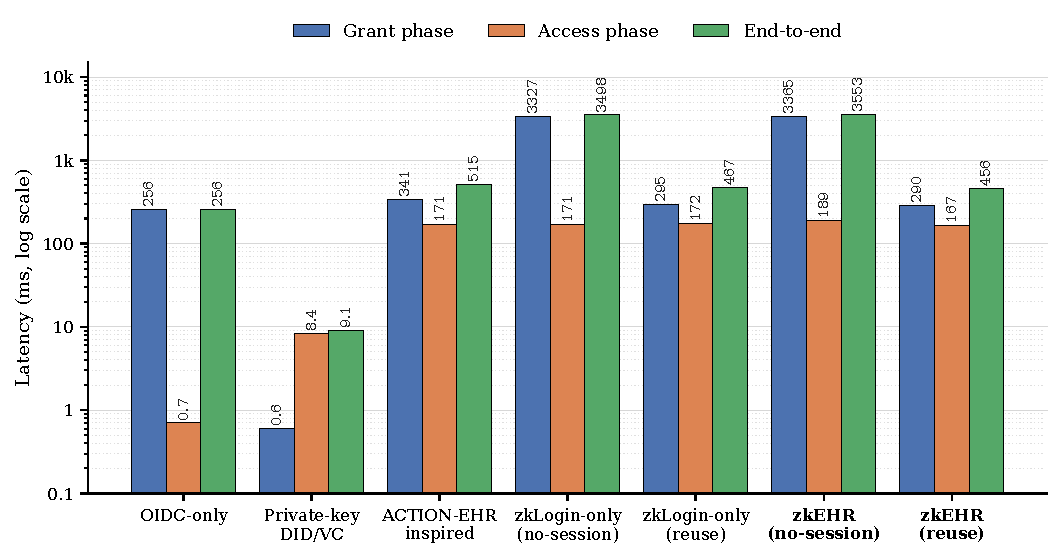
\includegraphics[width=0.95\textwidth]{cross_institution_latency.pdf}
\caption{End-to-end cross-institution access latency across five
architectures (mean of $n{=}100$ measured runs, log scale).
\textit{(no-session)} denotes that the patient performs the full
zkLogin authentication on every access; \textit{(reuse)} denotes that
the patient establishes a zkLogin session once and reuses the cached
proof for subsequent accesses within the bound \texttt{maxEpoch}
window. The proposed zkEHR variants are highlighted in bold on the
$x$-axis. zkEHR (reuse) matches the simpler on-chain access-control
baselines in per-access cost while delivering keyless recovery,
OIDC-anchored identity binding, and DID-portable consent.}
\label{fig:e2e-cross-institution-latency}
\end{figure*}

\paragraph{Cost of the zkEHR security guarantees.}
The defining features of zkEHR---multi-authority salt derivation for
keyless DID recovery and DID-bound AccessGrants for portable consent
authorization---are visible in two complementary regimes. In
no-session mode (every access pays a fresh zkLogin authentication),
multi-authority salt with $N{=}4$ co-located institutions running
concurrently completes in $5.4$\,ms total wall-clock time (slowest
single-authority response: $4.9$\,ms), only a few milliseconds more
than the single-authority alternative used by zkLogin-only. The
no-session end-to-end cost is dominated by the Mysten devnet prover
($\approx$$2.8$\,s producing the Groth16 proof), which is orthogonal
to multi-authority salt and identical for both zkLogin-based
architectures. In session-reuse mode, both phases A--D (the entire
zkLogin authentication, including the prover and the multi-authority
salt) are paid \emph{once} per epoch window and amortized across
unlimited subsequent accesses. The per-access cost then collapses to a
single Sui transaction submission plus two \texttt{getObject}
round-trips for AccessGrant and B-DID resolution---a working point at
which zkEHR's per-access overhead is essentially indistinguishable
from the simpler ACTION-EHR-inspired baseline ($1.2\%$ overhead from
the additional B-DID resolve), while still delivering keyless DID
recovery, OIDC-anchored identity binding, and DID-portable consent
features that none of the simpler baselines provide.
.
%
% Required preamble (add to your main .tex if not already present):
%   \usepackage{booktabs}
%   \usepackage{multirow}
%   \usepackage{graphicx}
%
% Figure dependency:
%   cross_institution_latency.pdf  (regenerate with: python3 plot_cross_institution_latency.py)
%   Place the .pdf alongside this .tex (or under your figs/ directory)
%   and update the \includegraphics path below if needed.
% =========================================================================

\subsubsection{End-to-End Cross-Institution Access Authorization and Verification Latency}
\label{sec:eval-e2e-cross-institution}

We evaluate the end-to-end latency of cross-institution Electronic
Health Record (EHR) access authorization and verification across five
architectural designs: a centralized OIDC consent registry
(\textit{OIDC-only}), a private-key DID/VC presentation model
(\textit{Private-key DID/VC}), an ACTION-EHR-inspired patient-centric
on-chain access-control baseline (\textit{ACTION-EHR-inspired}), a
zkLogin-driven on-chain access-grant baseline (\textit{zkLogin-only}),
and our proposed \textit{zkEHR} system, which combines DID-bound
on-chain AccessGrant objects, multi-authority salt derivation, and
zkLogin authentication. For the two zkLogin-based architectures we
report two operational modes: \textit{no-session} (the patient's
zkLogin credentials are derived from scratch on every access) and
\textit{session-reuse} (the patient establishes a zkLogin session once
and reuses the cached
$(\text{ephemeral key},\, \text{proof},\, \text{addressSeed},\,
\text{maxEpoch})$ tuple until the bound \texttt{maxEpoch} expires).

\paragraph{Experimental setup.}
All chain-touching baselines target Sui Devnet through the same Sui
Move \texttt{access\_grant} package, deployed once and shared across
baselines for fairness. The benchmarking host is a single Amazon EC2
instance in \texttt{us\nobreakdash-east\nobreakdash-1}, geographically
close to Sui's GCP-hosted devnet RPC endpoint
\texttt{fullnode.devnet.sui.io} ($\approx$1.5\,ms TCP RTT). For each
baseline we record 100 measured runs preceded by 10 warm-up runs that
are dropped from statistics. High-resolution timing uses
\texttt{process.hrtime.bigint()} (nanosecond resolution). Failed runs
are reported separately and excluded from latency percentiles. Sui
transactions use the \texttt{WaitForEffectsCert} submission semantics;
queries that target freshly-created objects use bounded retries to
absorb fullnode indexer lag (the wait is included in
\texttt{access\_grant\_query\_ms}, matching realistic e2e cost). For
zkEHR, multi-authority salt derivation uses $N{=}4$ co-located
authorities behind a parallel fan-out and a SHA-256 merge to a 128-bit
salt.

\paragraph{Results.}
Table~\ref{tab:e2e-cross-institution-latency} reports per-phase and
end-to-end latency for each baseline.
Figure~\ref{fig:e2e-cross-institution-latency} visualizes the
distribution on a logarithmic scale to span the four orders of
magnitude across baselines. We make five observations:

\begin{enumerate}
\item \textbf{Private-key DID/VC} achieves the lowest end-to-end
latency ($9.1$\,ms) because the patient signs the consent VC locally
and Hospital A issues a single chain query for DID resolution. However,
it provides no keyless recovery, no on-chain consent revocation
visibility, and no IdP-anchored identity binding.

\item \textbf{OIDC-only} attains the lowest \textit{access-side}
latency ($0.7$\,ms) since consent is centrally stored, but it incurs a
$255.6$\,ms federated-login cost on every grant operation because it
has no on-chain artifact and the consent registry is owned solely by
Hospital~A.

\item In \textbf{no-session mode}, both zkLogin-only ($3498.3$\,ms) and
zkEHR ($3553.3$\,ms) are dominated by the Mysten devnet prover request
that produces the Groth16 proof ($\approx$$2.8$\,s, $\approx$$80\%$ of
the end-to-end cost). Multi-authority salt with $N{=}4$ authorities
adds only $5.4$\,ms over single-authority salt, $0.15\%$ of the
no-session end-to-end cost.

\item In \textbf{session-reuse mode}, zkLogin-only ($466.9$\,ms),
zkEHR ($456.5$\,ms), and ACTION-EHR-inspired ($514.7$\,ms) converge
because they share the same dominant cost: a Sui transaction
submission ($\approx$$190$\,ms with \texttt{WaitForEffectsCert}) plus
one or two \texttt{getObject} round-trips ($\approx$$160$\,ms each,
including fullnode index lag for freshly-created objects).

\item \textbf{zkEHR adds only $5.7$\,ms} of B-DID resolution on top of
zkLogin-only-reuse---a $1.2\%$ access-time overhead---in exchange for
full DID-resolved authorization, portable consent semantics, and
keyless recovery support.
\end{enumerate}

% --------------------------- Table -----------------------------------------
\begin{table*}[!t]
\caption{End-to-end cross-institution access latency across five
architectures (mean$\,\pm\,$std., $n{=}100$ measured runs each, on Sui
Devnet via Amazon EC2 us-east-1). \textit{ns}=no-session;
\textit{r}=session-reuse.}
\label{tab:e2e-cross-institution-latency}
\centering
\renewcommand{\arraystretch}{1.25}
\begin{tabular}{l rrr l}
\toprule
\textbf{Baseline} & \textbf{Grant phase (ms)} & \textbf{Access phase (ms)} & \textbf{End-to-end (ms)} & \textbf{Notes} \\
\midrule
OIDC-only                       & $\phantom{0}255.6 \pm \phantom{00}27.4$ & $\phantom{000}0.7 \pm \phantom{0}0.1$  & $\phantom{0}256.3 \pm \phantom{00}27.5$ & Centralized consent DB \\
Private-key DID/VC              & $\phantom{0000}0.6 \pm \phantom{000}0.1$ & $\phantom{000}8.4 \pm \phantom{0}1.3$  & $\phantom{0000}9.1 \pm \phantom{000}1.3$  & Local VC sign; 1 DID-resolve RPC \\
ACTION-EHR-inspired             & $\phantom{0}340.8 \pm \phantom{00}80.3$ & $\phantom{0}171.1 \pm 78.4$ & $\phantom{0}514.7 \pm \phantom{0}117.9$ & On-chain grant + verify \\
zkLogin-only (\textit{ns})      & $3327.1 \pm 325.6$ & $\phantom{0}171.2 \pm 52.6$ & $3498.3 \pm \phantom{0}339.9$ & Fresh OIDC + prover per access \\
zkLogin-only (\textit{r})       & $\phantom{0}294.9 \pm \phantom{00}44.6$ & $\phantom{0}172.0 \pm 59.0$ & $\phantom{0}466.9 \pm \phantom{00}80.3$ & Cached zkLogin proof; 1 chain RPC \\
\textbf{zkEHR} (\textit{ns})    & $\mathbf{3364.6 \pm 350.0}$            & $\mathbf{188.6 \pm 61.3}$ & $\mathbf{3553.3 \pm 356.3}$ & Multi-auth salt + DID-bound \\
\textbf{zkEHR (ours,~\textit{r})} & $\mathbf{289.7 \pm \phantom{00}37.7}$ & $\mathbf{166.7 \pm 59.9}$ & $\mathbf{456.5 \pm \phantom{00}67.5}$ & Cached + DID-bound; 2 chain RPCs \\
\bottomrule
\end{tabular}
\end{table*}

% --------------------------- Figure ----------------------------------------
% Figure rendered by plot_cross_institution_latency.py (matplotlib);
% regenerate via: python3 plot_cross_institution_latency.py
\begin{figure*}[!t]
\centering
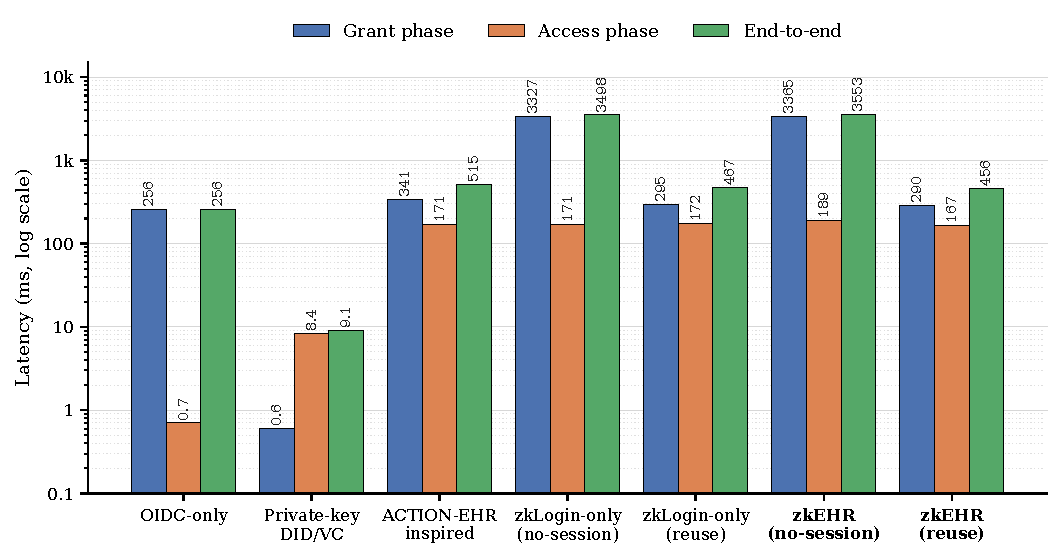
\includegraphics[width=0.95\textwidth]{cross_institution_latency.pdf}
\caption{End-to-end cross-institution access latency across five
architectures (mean of $n{=}100$ measured runs, log scale).
\textit{(no-session)} denotes that the patient performs the full
zkLogin authentication on every access; \textit{(reuse)} denotes that
the patient establishes a zkLogin session once and reuses the cached
proof for subsequent accesses within the bound \texttt{maxEpoch}
window. The proposed zkEHR variants are highlighted in bold on the
$x$-axis. zkEHR (reuse) matches the simpler on-chain access-control
baselines in per-access cost while delivering keyless recovery,
OIDC-anchored identity binding, and DID-portable consent.}
\label{fig:e2e-cross-institution-latency}
\end{figure*}

\paragraph{Cost of the zkEHR security guarantees.}
The defining features of zkEHR---multi-authority salt derivation for
keyless DID recovery and DID-bound AccessGrants for portable consent
authorization---are visible in two complementary regimes. In
no-session mode (every access pays a fresh zkLogin authentication),
multi-authority salt with $N{=}4$ co-located institutions running
concurrently completes in $5.4$\,ms total wall-clock time (slowest
single-authority response: $4.9$\,ms), only a few milliseconds more
than the single-authority alternative used by zkLogin-only. The
no-session end-to-end cost is dominated by the Mysten devnet prover
($\approx$$2.8$\,s producing the Groth16 proof), which is orthogonal
to multi-authority salt and identical for both zkLogin-based
architectures. In session-reuse mode, both phases A--D (the entire
zkLogin authentication, including the prover and the multi-authority
salt) are paid \emph{once} per epoch window and amortized across
unlimited subsequent accesses. The per-access cost then collapses to a
single Sui transaction submission plus two \texttt{getObject}
round-trips for AccessGrant and B-DID resolution---a working point at
which zkEHR's per-access overhead is essentially indistinguishable
from the simpler ACTION-EHR-inspired baseline ($1.2\%$ overhead from
the additional B-DID resolve), while still delivering keyless DID
recovery, OIDC-anchored identity binding, and DID-portable consent
features that none of the simpler baselines provide.
.
%
% Required preamble (add to your main .tex if not already present):
%   \usepackage{booktabs}
%   \usepackage{multirow}
%   \usepackage{graphicx}
%
% Figure dependency:
%   cross_institution_latency.pdf  (regenerate with: python3 plot_cross_institution_latency.py)
%   Place the .pdf alongside this .tex (or under your figs/ directory)
%   and update the \includegraphics path below if needed.
% =========================================================================

\subsubsection{End-to-End Cross-Institution Access Authorization and Verification Latency}
\label{sec:eval-e2e-cross-institution}

We evaluate the end-to-end latency of cross-institution Electronic
Health Record (EHR) access authorization and verification across five
architectural designs: a centralized OIDC consent registry
(\textit{OIDC-only}), a private-key DID/VC presentation model
(\textit{Private-key DID/VC}), an ACTION-EHR-inspired patient-centric
on-chain access-control baseline (\textit{ACTION-EHR-inspired}), a
zkLogin-driven on-chain access-grant baseline (\textit{zkLogin-only}),
and our proposed \textit{zkEHR} system, which combines DID-bound
on-chain AccessGrant objects, multi-authority salt derivation, and
zkLogin authentication. For the two zkLogin-based architectures we
report two operational modes: \textit{no-session} (the patient's
zkLogin credentials are derived from scratch on every access) and
\textit{session-reuse} (the patient establishes a zkLogin session once
and reuses the cached
$(\text{ephemeral key},\, \text{proof},\, \text{addressSeed},\,
\text{maxEpoch})$ tuple until the bound \texttt{maxEpoch} expires).

\paragraph{Experimental setup.}
All chain-touching baselines target Sui Devnet through the same Sui
Move \texttt{access\_grant} package, deployed once and shared across
baselines for fairness. The benchmarking host is a single Amazon EC2
instance in \texttt{us\nobreakdash-east\nobreakdash-1}, geographically
close to Sui's GCP-hosted devnet RPC endpoint
\texttt{fullnode.devnet.sui.io} ($\approx$1.5\,ms TCP RTT). For each
baseline we record 100 measured runs preceded by 10 warm-up runs that
are dropped from statistics. High-resolution timing uses
\texttt{process.hrtime.bigint()} (nanosecond resolution). Failed runs
are reported separately and excluded from latency percentiles. Sui
transactions use the \texttt{WaitForEffectsCert} submission semantics;
queries that target freshly-created objects use bounded retries to
absorb fullnode indexer lag (the wait is included in
\texttt{access\_grant\_query\_ms}, matching realistic e2e cost). For
zkEHR, multi-authority salt derivation uses $N{=}4$ co-located
authorities behind a parallel fan-out and a SHA-256 merge to a 128-bit
salt.

\paragraph{Results.}
Table~\ref{tab:e2e-cross-institution-latency} reports per-phase and
end-to-end latency for each baseline.
Figure~\ref{fig:e2e-cross-institution-latency} visualizes the
distribution on a logarithmic scale to span the four orders of
magnitude across baselines. We make five observations:

\begin{enumerate}
\item \textbf{Private-key DID/VC} achieves the lowest end-to-end
latency ($9.1$\,ms) because the patient signs the consent VC locally
and Hospital A issues a single chain query for DID resolution. However,
it provides no keyless recovery, no on-chain consent revocation
visibility, and no IdP-anchored identity binding.

\item \textbf{OIDC-only} attains the lowest \textit{access-side}
latency ($0.7$\,ms) since consent is centrally stored, but it incurs a
$255.6$\,ms federated-login cost on every grant operation because it
has no on-chain artifact and the consent registry is owned solely by
Hospital~A.

\item In \textbf{no-session mode}, both zkLogin-only ($3498.3$\,ms) and
zkEHR ($3553.3$\,ms) are dominated by the Mysten devnet prover request
that produces the Groth16 proof ($\approx$$2.8$\,s, $\approx$$80\%$ of
the end-to-end cost). Multi-authority salt with $N{=}4$ authorities
adds only $5.4$\,ms over single-authority salt, $0.15\%$ of the
no-session end-to-end cost.

\item In \textbf{session-reuse mode}, zkLogin-only ($466.9$\,ms),
zkEHR ($456.5$\,ms), and ACTION-EHR-inspired ($514.7$\,ms) converge
because they share the same dominant cost: a Sui transaction
submission ($\approx$$190$\,ms with \texttt{WaitForEffectsCert}) plus
one or two \texttt{getObject} round-trips ($\approx$$160$\,ms each,
including fullnode index lag for freshly-created objects).

\item \textbf{zkEHR adds only $5.7$\,ms} of B-DID resolution on top of
zkLogin-only-reuse---a $1.2\%$ access-time overhead---in exchange for
full DID-resolved authorization, portable consent semantics, and
keyless recovery support.
\end{enumerate}

% --------------------------- Table -----------------------------------------
\begin{table*}[!t]
\caption{End-to-end cross-institution access latency across five
architectures (mean$\,\pm\,$std., $n{=}100$ measured runs each, on Sui
Devnet via Amazon EC2 us-east-1). \textit{ns}=no-session;
\textit{r}=session-reuse.}
\label{tab:e2e-cross-institution-latency}
\centering
\renewcommand{\arraystretch}{1.25}
\begin{tabular}{l rrr l}
\toprule
\textbf{Baseline} & \textbf{Grant phase (ms)} & \textbf{Access phase (ms)} & \textbf{End-to-end (ms)} & \textbf{Notes} \\
\midrule
OIDC-only                       & $\phantom{0}255.6 \pm \phantom{00}27.4$ & $\phantom{000}0.7 \pm \phantom{0}0.1$  & $\phantom{0}256.3 \pm \phantom{00}27.5$ & Centralized consent DB \\
Private-key DID/VC              & $\phantom{0000}0.6 \pm \phantom{000}0.1$ & $\phantom{000}8.4 \pm \phantom{0}1.3$  & $\phantom{0000}9.1 \pm \phantom{000}1.3$  & Local VC sign; 1 DID-resolve RPC \\
ACTION-EHR-inspired             & $\phantom{0}340.8 \pm \phantom{00}80.3$ & $\phantom{0}171.1 \pm 78.4$ & $\phantom{0}514.7 \pm \phantom{0}117.9$ & On-chain grant + verify \\
zkLogin-only (\textit{ns})      & $3327.1 \pm 325.6$ & $\phantom{0}171.2 \pm 52.6$ & $3498.3 \pm \phantom{0}339.9$ & Fresh OIDC + prover per access \\
zkLogin-only (\textit{r})       & $\phantom{0}294.9 \pm \phantom{00}44.6$ & $\phantom{0}172.0 \pm 59.0$ & $\phantom{0}466.9 \pm \phantom{00}80.3$ & Cached zkLogin proof; 1 chain RPC \\
\textbf{zkEHR} (\textit{ns})    & $\mathbf{3364.6 \pm 350.0}$            & $\mathbf{188.6 \pm 61.3}$ & $\mathbf{3553.3 \pm 356.3}$ & Multi-auth salt + DID-bound \\
\textbf{zkEHR (ours,~\textit{r})} & $\mathbf{289.7 \pm \phantom{00}37.7}$ & $\mathbf{166.7 \pm 59.9}$ & $\mathbf{456.5 \pm \phantom{00}67.5}$ & Cached + DID-bound; 2 chain RPCs \\
\bottomrule
\end{tabular}
\end{table*}

% --------------------------- Figure ----------------------------------------
% Figure rendered by plot_cross_institution_latency.py (matplotlib);
% regenerate via: python3 plot_cross_institution_latency.py
\begin{figure*}[!t]
\centering
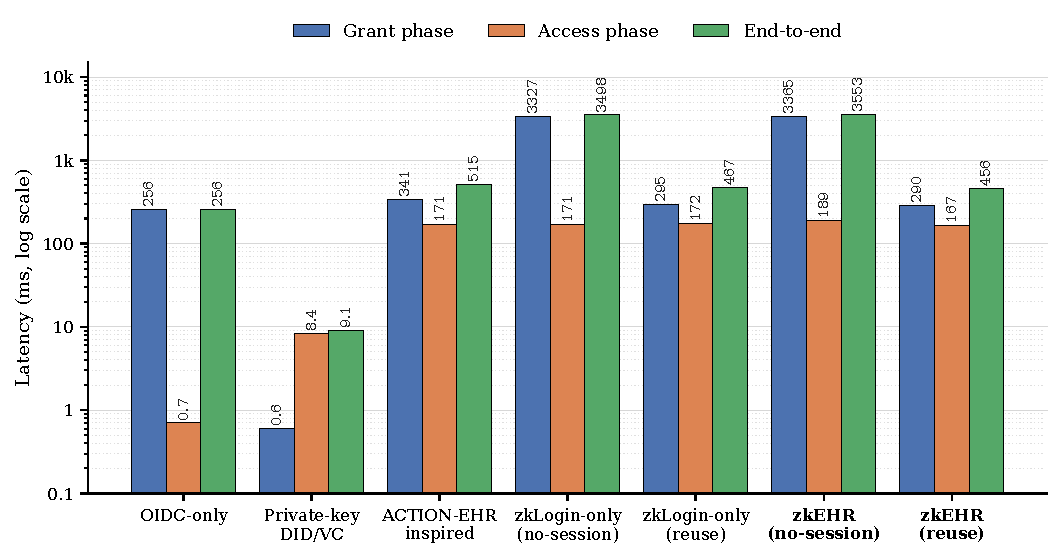
\includegraphics[width=0.95\textwidth]{cross_institution_latency.pdf}
\caption{End-to-end cross-institution access latency across five
architectures (mean of $n{=}100$ measured runs, log scale).
\textit{(no-session)} denotes that the patient performs the full
zkLogin authentication on every access; \textit{(reuse)} denotes that
the patient establishes a zkLogin session once and reuses the cached
proof for subsequent accesses within the bound \texttt{maxEpoch}
window. The proposed zkEHR variants are highlighted in bold on the
$x$-axis. zkEHR (reuse) matches the simpler on-chain access-control
baselines in per-access cost while delivering keyless recovery,
OIDC-anchored identity binding, and DID-portable consent.}
\label{fig:e2e-cross-institution-latency}
\end{figure*}

\paragraph{Cost of the zkEHR security guarantees.}
The defining features of zkEHR---multi-authority salt derivation for
keyless DID recovery and DID-bound AccessGrants for portable consent
authorization---are visible in two complementary regimes. In
no-session mode (every access pays a fresh zkLogin authentication),
multi-authority salt with $N{=}4$ co-located institutions running
concurrently completes in $5.4$\,ms total wall-clock time (slowest
single-authority response: $4.9$\,ms), only a few milliseconds more
than the single-authority alternative used by zkLogin-only. The
no-session end-to-end cost is dominated by the Mysten devnet prover
($\approx$$2.8$\,s producing the Groth16 proof), which is orthogonal
to multi-authority salt and identical for both zkLogin-based
architectures. In session-reuse mode, both phases A--D (the entire
zkLogin authentication, including the prover and the multi-authority
salt) are paid \emph{once} per epoch window and amortized across
unlimited subsequent accesses. The per-access cost then collapses to a
single Sui transaction submission plus two \texttt{getObject}
round-trips for AccessGrant and B-DID resolution---a working point at
which zkEHR's per-access overhead is essentially indistinguishable
from the simpler ACTION-EHR-inspired baseline ($1.2\%$ overhead from
the additional B-DID resolve), while still delivering keyless DID
recovery, OIDC-anchored identity binding, and DID-portable consent
features that none of the simpler baselines provide.
